\documentclass[12pt,twoside]{report}
\usepackage[utf8]{inputenc}
\usepackage{graphicx}
\usepackage{amsmath}
\usepackage{amsfonts}
%\usepackage[spanish]{babel}  %Cosas en español

% ---------------- Puntos decimales en lugar de comas para los numeros ---------------------------------
%\decimalpoint

%--------------------------------------------- Estilo de las paginas -----------------------------------
\usepackage[letterpaper,width=150mm,top=25mm,bottom=25mm,bindingoffset=6mm]{geometry}
\usepackage{fancyhdr}
\pagestyle{fancy}
\usepackage{multirow}
\usepackage{color}
\usepackage{colortbl}
\usepackage{xcolor}
\usepackage{float}
\definecolor{MSUgreen}{RGB}{0,150,150}
\fancyhead{}
\fancyhead[RE,LO]{\rightmark}
%\fancyhead[LE,RO]{\thepage}
\usepackage{bbold}
\fancyfoot{}
\fancyfoot[CE,CO]{\thepage}


\renewcommand{\headrulewidth}{0.4pt}

%\usepackage{biblatex}
%\addbibresource{chapters/bibliografía.bib}

%--------------------------Para las citas (al menos m comprime cuando son muchas y no las pone entre comas)
\usepackage{cite}
\usepackage{varioref}
\usepackage[breaklinks,colorlinks=true, pdfstartview=FitV, linkcolor=blue, citecolor=red, urlcolor=blue]{hyperref}
%\usepackage{kantlipsum}
\usepackage{textcomp}
\usepackage{subfigure}
\usepackage{appendix}
%\usepackage{cite}           % para contraer referencias
\usepackage{longtable}      % Utilizado para la lista de simbolos
\usepackage{fancyhdr}
\usepackage{color}
\usepackage{xcolor}
\usepackage{pstricks}
\usepackage{blkarray}
%----------------------------------- Para hacer indice en panel lateral ----------------------------------
\usepackage{hyperref}
%\hypersetup{pdftex,colorlinks=true,allcolors=blue}
\usepackage{hypcap}

%-------------------------- Paquete para modificar los titulos de los cap y secciones---------------------
\usepackage{titlesec}		

%------------------------------- Lineas alrededor de los capitulos numerados -----------------------------
\titleformat{\chapter}[display]
{\Large\bfseries}
{\titlerule[4pt] \chaptertitlename\ \thechapter}{5pt}
{\large}[{\titlerule[2pt]}]


%------------------------------- Lineas alrededor de los capitulos no numerados -----------------------------
\titleformat{name=\chapter,numberless}[display]
{\Large\bfseries}
{\titlerule[4pt]}{-20pt}
{\large}[{\titlerule[2pt]}]

\titlespacing*{\chapter}{0pt}{30pt}{20pt}

%\usepackage[nottoc,numbib]{tocbibind}


\graphicspath{ {./Figures/} }
\lhead{Modeling properties of the double exchange model hamiltonian}
\rhead{M2 Internship}
%\lfoot{TODO 1}
%\rfoot{TODO 1}
%\def\changemargin#1#2{\list{}{\rightmargin#2\leftmargin#1}\item[]}
%\let\endchangemargin=\endlist
\title{Modeling properties of the double exchange model hamiltonian}

\newcommand{\citepetsc}{\cite{petsc_web_page,petsc_user_ref,petsc_efficient}}
\newcommand{\citeslepc}{\cite{Hernandez_2003_SSL,slepc_users_manual}}





\begin{document}
	\begin{titlepage}
		\begin{center}
			%\vspace{-2cm}
			
\includegraphics[width = 0.2\textwidth]{lcpq.png} \hspace{0.5cm}
			
\includegraphics[width = 0.2\textwidth]{irsamac.png} \hspace{0.5cm}
			
\includegraphics[width = 0.2\textwidth]{ups.png} \hspace{0.5cm}
			
\includegraphics[width = 0.25\textwidth]{TCCM.png} \\
			\vspace{1cm}
			\Large
			{Master studies in Theoretical Chemistry and Computational Modelling\\
				Laboratoire de chimie et physique quantiques\\
				Université Toulouse III - Paul Sabatier\\
				%\end{center}
				
				%\includegraphics[width = 0.10\textwidth]{insteclogo} \hspace{2cm}
				
				%\includegraphics[width = 0.10\textwidth]{UH_logo.png} \\
				\vspace{-0.5cm}
				
				
				
				%\vspace{0.5cm}		
				
				
				
				\vspace{2cm}
				\Huge
				\textbf{ \color{MSUgreen} Modeling properties of the double exchange model hamiltonian }
				
				\vspace{3cm}
				\Large
				\begin{tabular}{l l}			
					{\bf Author:}   & Jos\'e David Crem\'e \\[1cm]
					{\bf Supervisors:} & Vijay G. Chilkuri \\
					& Nicolas Suaud
				\end{tabular}
			}
			
			\vspace{3cm}
			\Large
			Toulouse, 2023 \\
			
			\vspace{0.8cm}
			
		\end{center}
	\end{titlepage}
	%\maketitle
	\thispagestyle{empty}
	%\setcounter{page}{1}
	\tableofcontents
		\thispagestyle{empty}
	\chapter*{Introduction}
	\setcounter{page}{1}
	\setlength{\parskip}{-1mm}
	\addcontentsline{toc}{chapter}{Introduction}
	
	Colossal magnetoresistance (CMR) is the prperty of some materials to change their
	electric conductivity drastically under the presence of a magnetic field.
	This change could be by several orders of magnitude depending on the
	temperature and the amount of doping. This phenomenon has been observed
	mainly in manganites and nickelates under dopping, as shown in figure 1. The
	double exchange hamiltonian is usually used in order to model 1D chains of
	nickelates and the main objective of this work is to understand the
	microscopic origin of colossal magnetoresistance and the goal for the
	present master thesis is to analyse and understand some of the properties of
	the double exchange hamiltonian and its parameters.
	 
	\begin{center}
\begin{figure}[h!]
\hspace{1cm}
	\begin{minipage}{0.4\textwidth}
		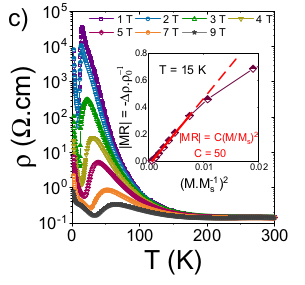
\includegraphics[scale=0.48]{i1.png}
	\end{minipage}
	\hspace{2.5cm}
		\begin{minipage}{0.4\textwidth}
			\includegraphics[scale=0.25]{i2.png}
		\end{minipage}
		%\includegraphics[scale=0.4]{../Graph/i2}		
\end{figure}
{\bf Figure 1:} Electrical resistivity measurements on: left: dopped Eu$_5$In$_2$Sb$_6$ single crystals. $\rho(T)$ at various magnetic fields applied \cite{1JD}. Right: $\rho$ vs magnetic field at various temperatures for (Sm$_{1-y}$Gd$_y)_{0.55}$Sr$_{0.45}$MnO$_3$, y=0.5 \cite{2JD}
\end{center}
	\section*{Experimental studies}
	\addcontentsline{toc}{section}{Experimental studies}
	
	One dimensional transition metal chains have been synthesized and studied in
	literature.~\cite{darriet_compound_1993,batlogg_haldane_1994} Experimental
	studies on 1D Nickelates have shown that they exhibit a magnetic field
	dependence in their resistivity upon doping.\cite{xu_holes_2000} Here, we
	focus on the low temperature behavior of the 1D doped Nickelates close to
	the curie temperature. Experimental studies of susceptibility of 1D doped
	Nickelates have shown that near the Curie temperature, the materials show
	antiferromagnetic behavior.\cite{Ramirez} This behavior is contrary to the
	usual double exchange model where the holes are supposed to be mobile
	throughout the chain. We develop arguments and discuss some new ideas to
	explain this behavior of the magnetic susceptibility in 1D doped Nickelates.
	
	\section*{Theoretical studies}
	\addcontentsline{toc}{section}{Theoretical studies}
	
	One dimensional transition metal chains are immencely useful models for
	theoretical analysis due to the existance of powerful techniques such as the
	density matrix renormalization group (DMRG) and lanczos exact
	diagonalization techniques. Such methods can be applied to high accuracy and
	have been used to study models similar to the one
	studied.\cite{dagotto_correlated_1994,patel_emergence_2020} Further work by
	Dagotto. et. al have shown details of the existance of a ferromagnetic
	polaron and its extent in such 1D models.\cite{malvezzi_origin_2001}
	However, the present study differs significantly from those cited above in
	two important ways. First, the parameter range that we have chosen for the
	current study relies on those extracted by \textit{ab initio} calculstions
	on Nickel dimers.\cite{bastardis_microscopic_2007,bastardis_isotropic_2008}
	Second, we use exact diagonalisation to be able to obtain a large number of
	low lying states for challenging parameter values which is a difficult task
	to acomplish even via DMRG techniques. Therefore, the present study serves
	to augment the available literature for parameter range extracted using
	\textit{ab initio} calculations.
	
	\chapter{Methodology}
	\section{Double Exchange Hamiltonian}
	The double exchange model is used to describe mixed lvalent transition
	metal based molecules. The phenomenology of ferromagnetic and anti-ferromagnetic
	behavior in such molecules is captured by the various parameters of the
	double exchange model Hamiltonian (Eq:~\ref{eq:demodel1}).
	
	\begin{equation}
		%\begin{split}
			\hat{H}  = \sum_i 2K \hat{S}_{a_i}\cdot\hat{S}_{b_i} 
			+ \sum_{ij} 2J_a \hat{S}_{a_i}\cdot\hat{S}_{a_j} 
			+ \sum_{ij} t\left( \hat{c}^{\dagger}_{a_i}\cdot\hat{c}_{a_j} + \text{h.c.}\right )
		%&	+ \sum_{i,i+1} V_{NN}\left ( \delta_{n_i,0}\ \delta_{n_{i+1},0} \right ) 
		%	+ \sum_{i,i+2} V_{NNN}\left ( \delta_{n_i,0}\ \delta_{n_{i+2},0} \right )
		%\end{split}
		\label{eq:demodel1}
	\end{equation}
	
	The main phenomenology that is incorporated in the hamiltonian is the
	competition between the parallel alignment of the electrons favored by the
	kinetic-energy term $t$ and the anti-parallel alignment favored by the
	potential term $J$. This competition gives rise to a rich phase diagram
	which might give rise to the phenomenology of CMR.

	In the present work we have also incorporated the hole repulsion as proposed
	by C. J. Calzado and J.  P. Malrieu \cite{calzado_proposal_2001}, this
	repulsion is considered beteenw two consecutive holes (Eq.
	\ref{eq:demodel2}).
	\begin{equation}
		\begin{split}
			\hat{H} & = \sum_i 2K \hat{S}_{a_i}\cdot\hat{S}_{b_i} 
			+ \sum_{ij} 2J_a \hat{S}_{a_i}\cdot\hat{S}_{a_j} 
			+ \sum_{ij} t\left( \hat{c}^{\dagger}_{a_i}\cdot\hat{c}_{a_j} + \text{h.c.}\right ) \\
		&	+ \sum_{i,i+1} V_{NN}\left ( \delta_{n_i,0}\ \delta_{n_{i+1},0} \right ) 
		\end{split}
		\label{eq:demodel2}
	\end{equation}
	A second approximation to hole repulsion has been used considering repulsion
	between all the holes as a function of the distance (Eq. \ref{eq:demodel3}).
	\begin{equation}
		\begin{split}
			\hat{H} & = \sum_i 2K \hat{S}_{a_i}\cdot\hat{S}_{b_i} 
			+ \sum_{ij} 2J_a \hat{S}_{a_i}\cdot\hat{S}_{a_j} 
			+ \sum_{ij} t\left( \hat{c}^{\dagger}_{a_i}\cdot\hat{c}_{a_j} + \text{h.c.}\right ) \\
		&	+ \sum_{i,j} V_{ij}\left ( \delta_{n_i,0}\ \delta_{n_{j},0} \right )
		\end{split}
		\label{eq:demodel3}
	\end{equation}
	
	
	
	\begin{figure}[ht]
		\centering
			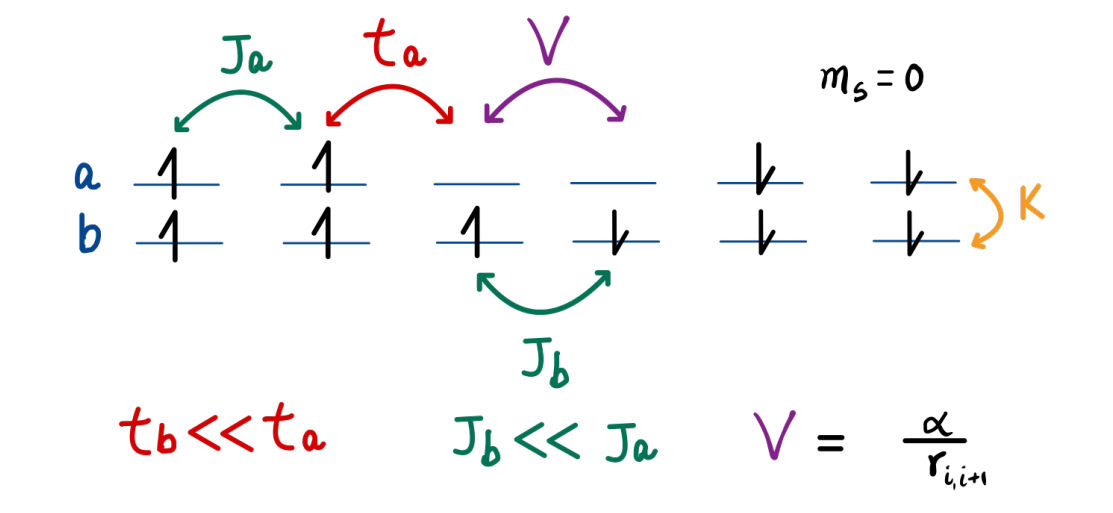
\includegraphics[scale=0.2]{DE.png}
		\caption{\label{fig:deham} Representation of a model system showing the interatction terms used in double exchange hamiltonian. }
	\end{figure}
	These Hamiltonians describe a model with two valence orbitals on each
	atom (site) ideally of differnet symmetry (i.e. orthogonal, e.g. $a,b$). A schematic is shown in
	Figure:~\ref{fig:deham}.
	%\begin{figure}[ht]
	%	\centering
	%	\begin{modiagram}[names]
	%		\atom[$1$]{left}{
	%			1s = { 0; up} ,
	%			2s = { 1; up} ,
	%		}
	%		
	%		\atom[$2$]{right}{
	%			1s = { 0; up} ,
	%			2s = { 1;   } ,
	%		}
	%		\node[right,xshift=4mm] at (1sright) {$b$};
	%		\node[right,xshift=4mm] at (2sright) {$a$};
	%		\node[left,xshift=-4mm] at (1sleft) {$b$};
	%		\node[left,xshift=-4mm] at (2sleft) {$a$};
	%		
	%		\draw[<-,gray,semithick]   (2sright) edge[bend right] node [left] {} (2sleft);
	%		\draw[<->,gray,semithick] (1sright) edge[bend left] node [left] {} (1sleft);
	%		\draw[<->,gray,semithick] (1sleft) edge[bend left] node [left] {} (2sleft);
			
	%		\node[left,xshift=2.3cm, yshift=-9mm] at (1sleft) {$J$};
	%		\node[left,xshift= 4mm, yshift=5mm] at (1sleft) {$K$};
	%		\node[left,xshift=2.3cm, yshift=-0mm] at (2sleft) {$t$};
			
	%	\end{modiagram}
	%	\caption{\label{fig:deham} Orbital diagram representing the mail interactions of the double exchange model with two valence orbitals on each atom.}
	%\end{figure}&
	%\newpage
	In Eq: \ref{eq:demodel1},\ref{eq:demodel2} and \ref{eq:demodel3} the spins of the electrons are represented by $S_a$,
	where the subscript $a$ denotes the orbital on which the electron resides.  The
	creation and annahilation operators of electrons are represented by
	$\hat{c}^{\dagger}$ and $\hat{C}$ respectively. The parameters in the model
	Hamiltonian are defined as follows:
	
	\begin{itemize}
		
		\item $K$ - The local exchange integral. This exchange integral
		  represents Hund's rule and is always positive. The local exchange
		  favors parallel coupling i.e. a local high spin determinant.
		
		\item $J$ - The kinetic exchange interaction between orbitals of
		  symmetry $a$ on neighboring sites. This interaction is responsible of
		  the anti-parallel coupling.
		
		\item $t$ - The kinetic energy term or the hopping term. The transfer of
		  electrons from one atom to the neighboring atom is represented by the
		  hopping term. This also favors parallel coupling when taken along with
		  the exchange integral $K$.
		
		\item $V$ - The hole repulsion term. This takes into account the
		  repulsion between holes which are on neighboring sites $V_{NN}=\alpha
		  \slash 2$ or all the sites as a function of distance $V_{ij}=\alpha
		  \slash 2r_{ij}$. The hole repulsion indirectly takes into account the
		  repulsion between electrons.\cite{calzado_proposal_2001}
		
	\end{itemize}

	Note that in the present model, we assume a distance of 1 a.u. between adjascent
	sites which implies that $r_{ij} = |i-j|$ a.u.
	
	It is important to emphasize again that there is a competition between $J$ which favors the antiferromagnetic couplings and $t$ which favors the ferromagnetic couplings, this competition plays a fundamental rol in the physics of the system.
	
	\section{Parameter Space}
	
	All the parameters of the model are important for understanding the
	collective properties of the double exchange hamiltonian. Here we give the
	order of magnitude of all the parameters used keeping in mind that we target
	molecules based on transition metal atoms.  Previous studies using
	\textit{ab initio} methods in order to extract model parameters for various
	transition metal atoms such as Cu, Mn, and Ni have provided realistic order
	of magnitudes of the values of the parameters.  In the present analysis, we
	use the full range of values in order to represent the full range of
	transition metal atoms.
	
	\begin{table}[h!]
		\centering
		\begin{tabular}{||c||}
			\hline
			Parameters  \\ [0.5ex]
			\hline\hline
			\\
			$ -0.2|t|\lvert t \rvert \le J \le 0|t|\lvert t \rvert $    \\ [1ex]
			%$ 0.01\lvert t \rvert \le J \le 0.15\lvert t \rvert $    \\ [1ex]
			$  K = 0.8 |t| $                                    \\ [1ex]
			$ V_{NN} = \frac{\alpha}{2}\ ;\ 0.0|t| \le \frac{\alpha}{2} \le 5.0|t| $ \\ [1ex]
			$ V_{ij} = \frac{\alpha}{2r_{ij}} ;\ 0.0|t| \le \frac{\alpha}{2} \le 5.0|t|$                                \\ [1ex]
			\hline
		\end{tabular}
		\label{tab:params}
		\caption{Table with range of parameter values used in our calculations.}
	\end{table}
	
	Including the hole repulsion term significantly changes the low energy physics
	of the model as shown by previous work\cite{calzado_proposal_2001}. Here we will
	study the influence in the variation of some of the above parameters.
	
	
	%\chapter{Methodology}
	
	The double exchange hamiltonian is studied for one dimensional chain of
	sites containing holes with a doping ratio of 1:3 i.e. one hole for every
	three sites, from now the notation $n_{l\text{h}}$ will be used to refer a chain
	with $n$ sites and $l$ holes. This follows the previous study by V. G.
	Chilkuri which shows that for the physically meaningful range of parameter
	values, a single hole aligns about three sites.\cite{crystals_chilkuri}
	
	\section{Exact diagonalization}
	
	An exact diagonalization method is used to obtain many low energy states of
	the hamiltonian. Due to the exponential growth of the hilbert space with the
	number of sites, exact diagonalization becomes challenging. Here we use our
	home made code relying on PETSc\citepetsc and SLEPc\citeslepc libraries to
	perform exact diagonalization and use a large number of high performance
	compute nodes for distributed storage of the hamiltonian matrix and
	eigenvectors. We have used DEHam\cite{DEHamam} to perform exact
	diagonalization of very large number of sites up to 18 sites containing 36
	orbitals with 6 holes which corresponds to a hilbert space of about $0.5
	\times 10^9$ determinants.
	
	\section{Model space}
	\begin{figure}[ht]
		\centering
			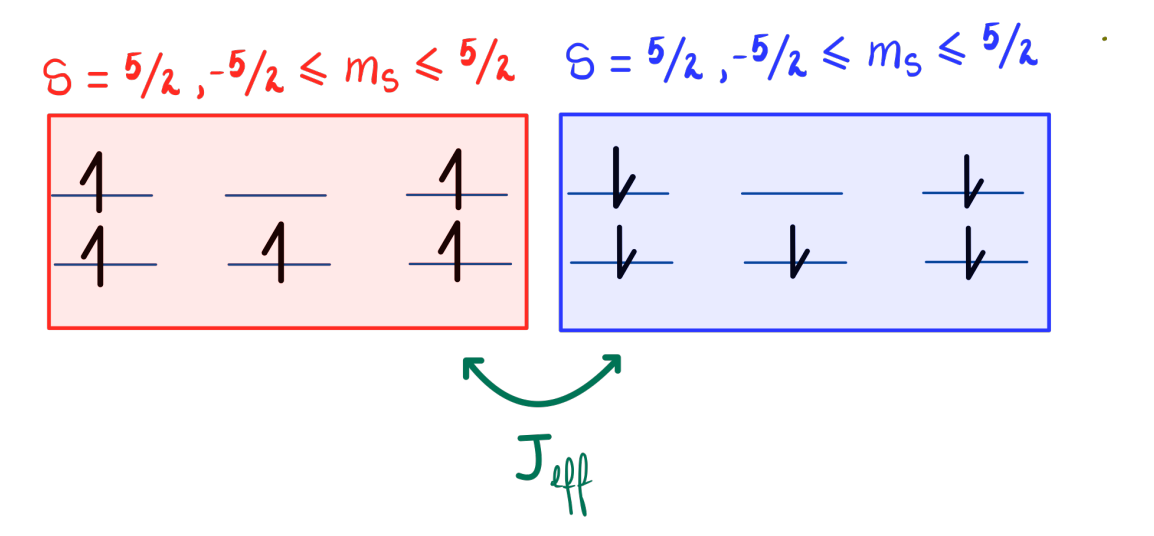
\includegraphics[scale=0.2]{boites.png}
		\caption{\label{boites}. Representation of the local ferromagnetic polarons formed by spins aligned by a single hole for 6$_{2h}$.}
	\end{figure}
	As discussed above, a hole aligns about three sites. That allows one to
	model the system considering "boxes" of 3 sites with a hole as a new "site"
	occupied by a particle with  $S=5 \slash 2$. These boxes have a
	ferromagnetic coupling inside and are coupled to each other in an
	anti-parallel or parallel way, as it is represented in figure \ref{boites}.
	Then, the model space is formed by all the possible determinats of the a
	chaing of $S=5 \slash 2$ spins. Some questions arise from this model:
	\begin{itemize}
	    \item Is the model space good enough (i.e. properly chosen) ?
	    \item For which range of values of $J$ do we obtain such a model space ?
	    \item What is the influence of hole repulsion ?
	    \item What is the model hamiltonian that reproduces the low energy spectrum ?
	\end{itemize}
	These are the questions that will be discussed in this report.
	
	
	\section{Model Hamiltonian}
	In this work we use a simple Heisemberg hamiltonian as a proposed model hamiltonian:
	\begin{equation}
	\hat{H}_{model}=-2J_{eff}\sum_i (\hat{S}_i\hat{S}_{i+1}-\frac{25}{4}\mathbb{1})
	\end{equation}
	Using Efective hamiltonian theory \cite{heff} to obtain a numerical hamiltonian which reproduce the double exchange wavefunction in the model espace, $J_{eff}$ can be calculated by fitting the analitical model hamiltonian to the effective hamiltonian.

	\section{Projector}

	Since here, we analyse the part of the wavefunction in the model space, a
	projector on the model space needs to be defined. Such a projector will
	project on determinants which contain only one hole inside a box containing
	three sites defined earlier. The projector must also project to a $S=5
	\slash 2$ spin inside the box. Therefore, the projector contains two parts,
	one spatial ($\hat{\mathcal{P}}_{space}$) projecting the hole positions and
	a second spin ($\hat{\mathcal{P}}_{spin}$) which takes care of the total
	spin inside the box. The total projector will be the product of these
	two projectors.

	\subsection{Spatial part}

	The spatial part of the projector is taken from the diagonalization of a
	Hueckel hamiltonian for three sites which is given below:

	\begin{equation}
      \begin{blockarray}{cccc}
      & \|bc\rangle & \|ac\rangle & \|ab\rangle \\
      \begin{block}{c(ccc)}
        \|bc\rangle & 0 & t & 0 \\
        \|ac\rangle & t & 0 & t \\
        \|ab\rangle & 0 & t & 0 \\
      \end{block}
      \end{blockarray}
		\label{eq:demodel}
	\end{equation}

	The basis are the three determinants possible for on hole and two particles,
	i.e. $|bc\rangle,|ac\rangle,|ab\rangle$.  Diagonalization of this
	hamiltonian gives the lowest energy eigenvector given below, which is used
	as the projector for the spatial part of the wavefunction inside each region
	composed of one hole and three sites.

	\begin{equation}
		\begin{split}
		  |\phi_{i}\rangle = \frac{1}{2}\left| bc\right\rangle +
\frac{\sqrt{2}}{2}\left| ac\right\rangle +
\frac{1}{2}\left| ab\right\rangle
		\end{split}
		\label{eq:demodel}
	\end{equation}


	The full projector is simply the tensor product of the above projector
	on all the box regions given as follows.

	\begin{equation}
		\begin{split}
			\hat{\mathcal{P}}_{space} & = \bigotimes_{i = 1}^{m}\left|\phi_i\right\rangle
		\end{split}
		\label{eq:demodel}
	\end{equation}

	\subsection{Spin part}

	The spin part of the projector for two sites is defined as follows:


	\begin{equation}
			\hat{\mathcal{P}}_{spin}(M_{S_T})  = \sum_{\substack{M_{S_1},M_{S_2}, \\ M_{S_1}+M_{S_2}=M_{S_T}}}
			\binom{5}{5 - 2 M_{S_1}}^{-1/2}\binom{5}{5 - 2 M_{S_2}}^{-1/2}
			\left |\frac{5}{2},M_{S_R}\right\rangle\otimes\left|\frac{5}{2},M_{S_L}\right\rangle
		\label{eq:demodel}
	\end{equation}

	where $S_T$ and $M_{S_T}$ represent the total spin and the total z component
	of the spin moment ($Ms$) respectively. The values $M_{S_1}$ and $M_{S_2}$
	represent the $Ms$ of the first and second $\frac{5}{2}$ spins respectively.
	The values in brackets represent binomial coefficients for each of the
	individual spins entering the product.

	Similarly, the projector for an arbitrary number of sites si similarly defined
	as follows:

	\begin{equation}
		\begin{split}
			\hat{\mathcal{P}}_{spin}(M_{S_T}) & = \sum_{\substack{M_{S_1}\dots M_{S_m},\\ M_{S_1} + \dots + M_{S_m} = M_{S_T}}} \prod_{i}^{m}
			\binom{5}{5 - 2 M_{S_i}}^{-1/2}
			\bigotimes_{i = 1}^{m}\left|\frac{5}{2},M_{S_i}\right\rangle
		\end{split}
		\label{eq:demodel}
	\end{equation}

    The wavefunction is a tensor product of all the possible $Ms$ combinations
	generated by $m$ ($\frac{5}{2}$) spins respecting the identity
	$\sum_i^m M_{S_i} = M_{S_T}$.  In this way, the spin part of the projector on the
	model space can be uniquely defined for an arbitrary number of sites.

	The total projector can then be written as the product of the spin
	and spatial parts given above.

	\begin{equation}
		\begin{split}
			\hat{\mathcal{P}} & = \hat{\mathcal{P}}_{space}\otimes\hat{\mathcal{P}}_{spin}
		\end{split}
		\label{eq:demodel}
	\end{equation}

	Note that the projector is normalized i.e.
	$\hat{\mathcal{P}}\cdot\hat{\mathcal{P}} = \hat{\mathcal{P}}$.

	\section{Effective Hamiltonian}

	Let $\hat{H}$ be the original hamiltonian describing a quantum system in
	an space of $N$ determinants, It has, therefore, $N$ eigenvalues and $N$
	eigenstates which fulfill the time-independent Schrödinger equation :

	\begin{equation}
	    \hat{H} |\Psi_I\rangle=E_I|\Psi_I\rangle
	\end{equation}

	Then, it is possible to define an effective hamiltonian $\hat{H}_{eff}$ which
	acts on a subspace of reduced dimensionality $n, n<N$, called the model space,
	and reproduces the $n$ exact eigenvalues of the original hamiltonian
	$\hat{H}$.

	\begin{equation}
	    \hat{H}_{eff} |\tilde{\Psi}_I\rangle=E_I|\tilde{\Psi}_I\rangle;\ 1 \le I \le n
	\end{equation}

	This states $|\tilde{\Psi}_n\rangle$ are the projected and orthonormalized
	components of $n$ states of the original hamiltonian $|\Psi_N\rangle$, onto
	the model space.  Projection of the original vectors on the model space can
	be obtained by applying the projector defined in the previous section:

	\begin{equation}
	    |\Phi_n\rangle=\hat{\mathcal{P}}|\Psi_N\rangle
	\end{equation}

	Then the weight of the "complete" wavefunction in the model space is defined as:

	\begin{equation}
	    W_i =\langle \Phi_i|\Phi_i\rangle
	\end{equation}

	It is evident that the set of states $|\Phi_n\rangle$ are not orthogonal nor
	normalized, but they can be orthonormalized following the procedure proposed
	by  des Cloizeaux \cite{Cloizeaux} as we show in what follows.

	Let us define the overlap matrix $S$ as $S_{ij} = \langle \Phi_i |
	\Phi_j\rangle$.  This matrix has as diagonal elements the weights of each
	$|\Psi_N\rangle$.  The weights of the projection for each state can also be
	defined as  $W_i=S_{ii}$.  The weight matrix can be expressed in terms of a
	diagonal matrix $D$ with diagonal elements $d_{ii} = S_{ii}$. One can
	diagonalize the overlap matrix to obtain the eigenvalues and eigenvectors as
	follows.

	\begin{equation}
	    S=U^{-1}DU
	\end{equation}

	Then a new diagonal matrix $D^{-1\slash 2}$ is computed with diagonal
	elements $d^{-1\slash 2}_{ii}=\dfrac{1}{\sqrt{d_{ii}}}$, then:

	\begin{equation}
	   S^{-1\slash 2}=U^{-1}D^{-1\slash 2}U 
	\end{equation}

	Hence, it is possible to show that a new orthonormal set of states can be
	obtained as expressed in eq. \ref{eq:orthonormal}:

	\begin{equation}
	   |\tilde{\Psi}_n \rangle=S^{-1 \slash 2}|\Phi_n \rangle
	   \label{eq:orthonormal}
	\end{equation}

	Now the effective hamiltonian is defined as:

	\begin{equation}
	    \hat{H}_{eff}=\langle \tilde{\Psi} | \mathbf{E} | \tilde{\Psi} \rangle
	\end{equation}

	Where $\tilde{\Psi}$ is a matrix formed by all the states $|\tilde{\Psi}_n\rangle$ and $E$ is a
	diagonal matrix having as diagonal elements the eigenstates of the target
	space.

	%\section{Real Space Renormalization Group}
	
	\begin{chapter}{Results and discussion}
	
	%\section{Hole repulsion}
	
	%TODO
	
	\section{Weight vs $J$}
	\subsection{Variation with the number of sites}
	\begin{figure}[ht]
		\centering
		\hspace{-2cm}
		\begin{minipage}{0.4\textwidth}
			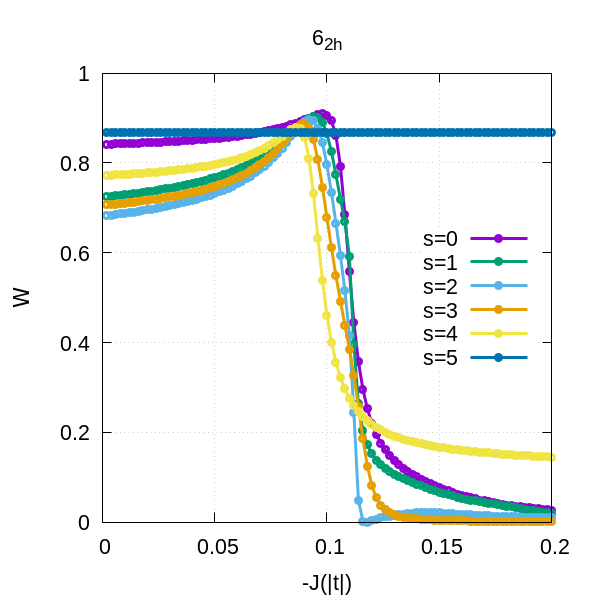
\includegraphics[scale=0.3]{W_vs_J_sites_2-xrep-0.png}
		\end{minipage}
		\hspace{2cm}
		\begin{minipage}{0.4\textwidth}
			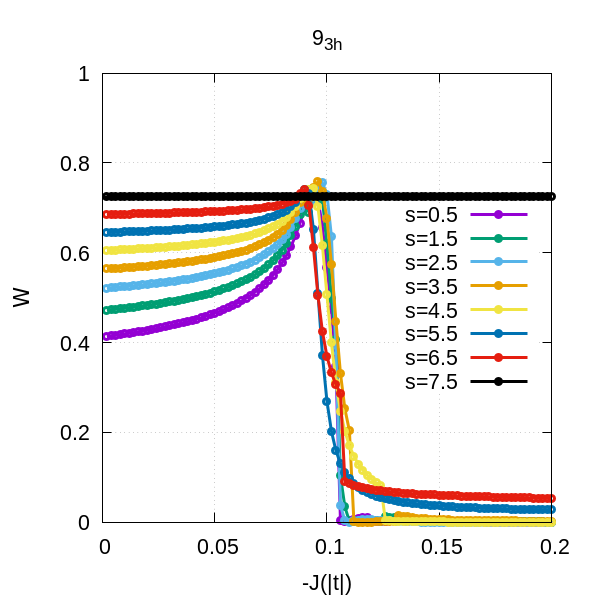
\includegraphics[scale=0.3]{W_vs_J_sites_3-xrep-0.png}
		\end{minipage}
		\caption{\label{fig_w69} Weight (W) as a function of $J$ for 6$_{2h}$ (left) and 9$_{3h}$ (right). }
	\end{figure}
	Figure \ref{fig_w69} shows the weight of the wave function projected in the
	model space as afunction of J for 6$_{2h}$ (left) and 9$_{3h}$ (right), for
	each spin sector, the state with the largest weight is chosen. This confirms
	that it is possible to have an interval of values of J in which the weight
	reaches satisfactory values (even $>$ 90$\%$ in some cases). It is easy to
	observe that the weights for 9$_{3h}$ are smaller than those of 6$_{2h}$.
	This due to the fact that with increasing size of the system and
	normalization of the wavefunction, the absolute weight of the model space
	decreases. In other words, the ratio of the size of the model space vs the
	total size of the Hilbert space goes to zero with increasing number of sites.
	
	\begin{figure}[h!]
		\centering
			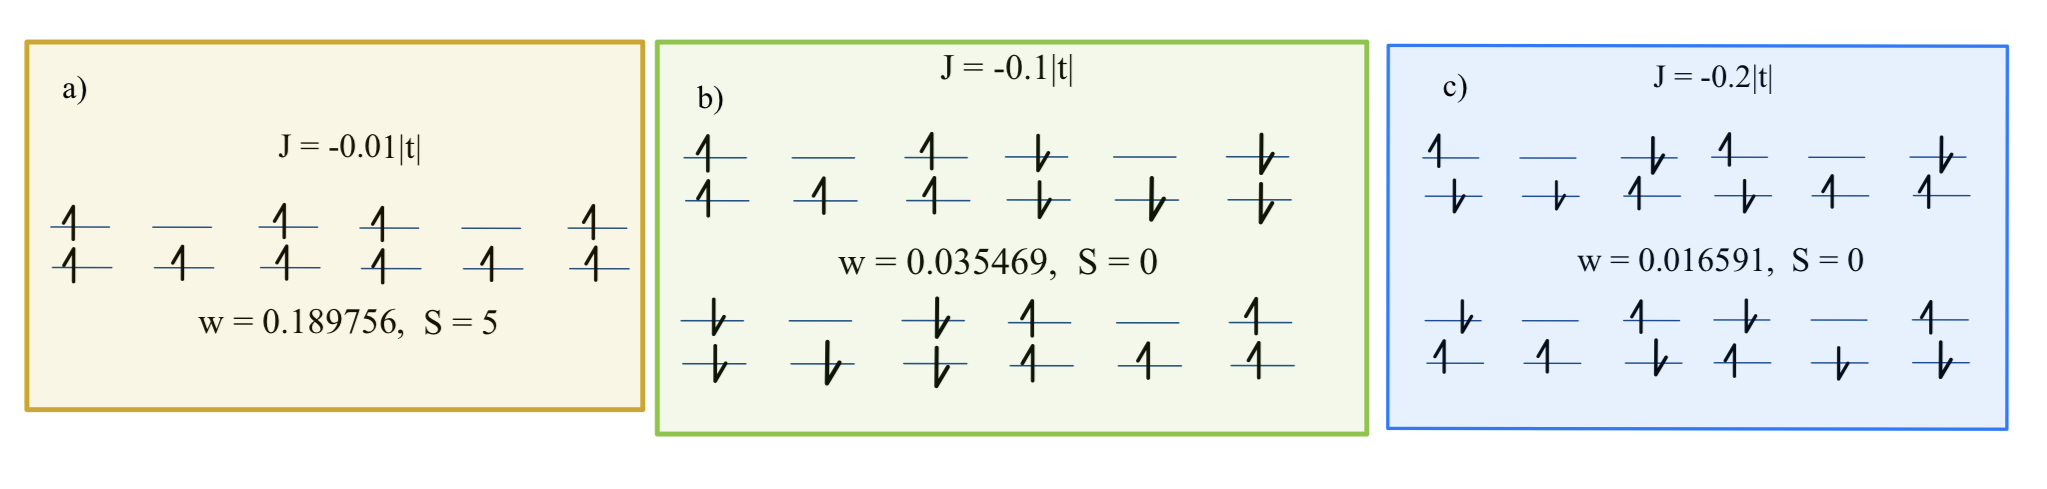
\includegraphics[scale=0.22]{determinants.jpg}
		\caption{\label{determinants}. Representation of the determinants with maximal weight on the ground state for three different values of $J$ in 6$_{2h}$.}
	\end{figure}
	 
	 Initially, the weight increases with increasing magnitude of $J$ this is
	 because for a small value of $J$ the system is completely governed by $t$
	 which will favor the ionic determinants. Howeveer, after a maximum, the
	 weight falls drastically as larger values of $J$ favors the
	 antiferromagnetic couplings inside the boxes and hense the component due to spin $S=5 \slash 2$ decreases. In order to ilustrated this figures \ref{determinants} shows the determinants with maximal weight on the ground state for three different values of $J$, in a) for $J=0.01|t|$, a very small values, the ground state is $S=5$ and the determinant having the maximal weight is all the electrons aligned and the hole in the middle of each box, as the Hückel wavefunction predicts. Then in b) for $J=0.1|t|$, an intermediate value, even if inside the boxes ferromagnetic coupling is favored the coupling between them is antiferromagnetic and the ground state is $S=0$. Finally, in c) when $J=0.2|t|$, a large value, there is no longer ferromagnetic coupling between the boxes.	
	
	\subsection{Variation with Repulsion}

	\begin{figure}[h!]
		\centering
		\hspace{-2cm}
		\begin{minipage}{0.4\textwidth}
			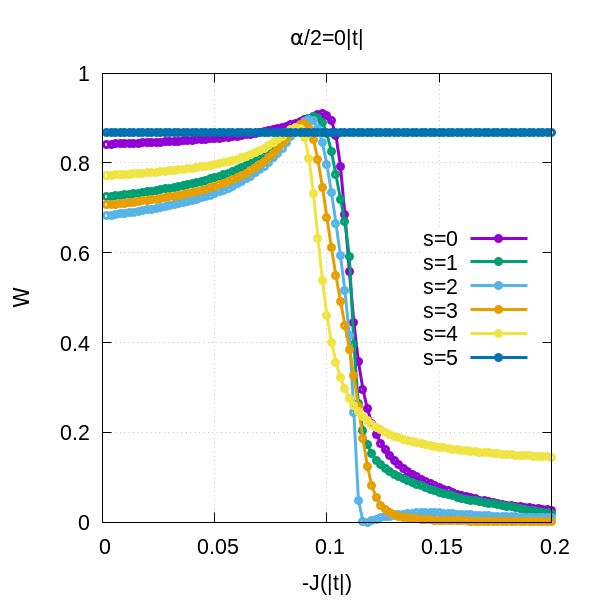
\includegraphics[scale=0.3]{W_vs_J_sites_2-xrep-01.png}
		\end{minipage}
		\hspace{2cm}
		\begin{minipage}{0.4\textwidth}
			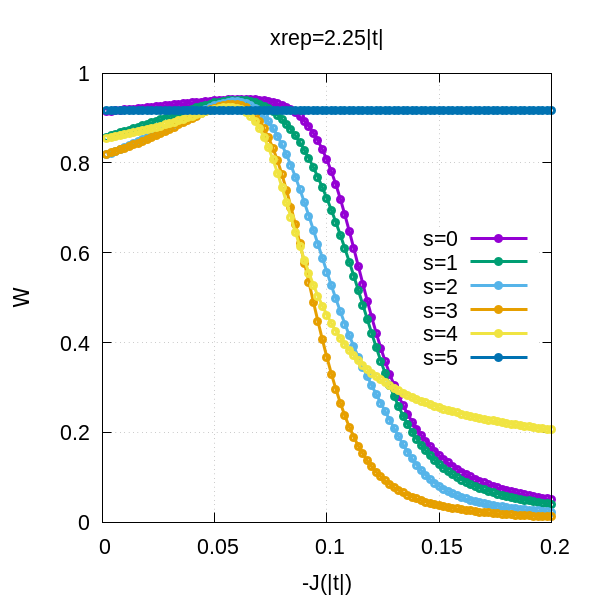
\includegraphics[scale=0.3]{W_vs_J_sites_2-xrep-225.png}
		\end{minipage}
		\caption{\label{fig_0_225} Weight (W) as a function of $J$ for $\alpha = 0 |t|$ (left) and $\alpha \slash 2 = 2.25|t|$ (right). }
	\end{figure}
	
	Figure \ref{fig_0_225}, shows the weight as a function of $J$ without hole
	repulsion (left) and with hole repulsion with $\alpha=2.25|t|$ (right). Here it
	is possible to see the same tendency but repulsion increases the weight in
	the model space as it forces the holes away from each other and this
	decreases the weight of the ionic determinants. This was one of the
	motivations to include the hole repulsion in the double exchange hamiltonian.

	\subsection{Conclusions}

	From the analysis above it is possible to conclude that the wavefunction has
	an excellent weight on the model space for $0.05 \leq J < 0.1|t|$

	\section{Influence of hole repulsion}

	\subsection{Variation of maximal weight}

	In order to better understand the effect of hole repulsion it is convenient
	to analize the maximal value of weight for each state for several values of
	$\alpha$ as displayed in figure \ref{fig_v1n} for two models: at left only
	considering repulsion between first neighbors and at right repulsion between
	all the holes as a function of the distance. At the begining there is an
	increase of the weight as explained above but for bigger values of repulsion
	there is a slight decrease as it will force the holes to be at the borders,
	and the spatial projector is the solution of Hückel in wich the hole at the
	exterior border of each box has a weight of 25$\%$, so even if it gains in
	weight the decreasing of the others components will cause a global but
	slight decrease. Therefore, we observe a maximum value of the weight for the
	values of $\alpha=2.25|t|$.
	
	\begin{figure}[h!]
		\centering
		\hspace{-2cm}
		\begin{minipage}{0.4\textwidth}
			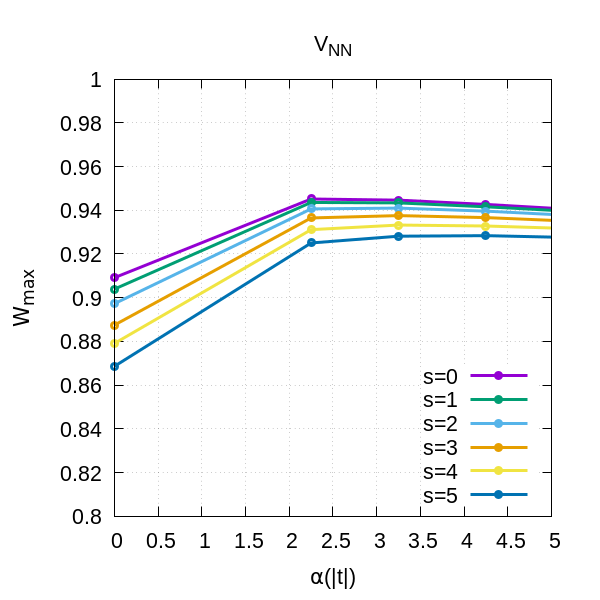
\includegraphics[scale=0.3]{Wmax_vs_xrep0v1.png}
		\end{minipage}
		\hspace{2cm}
		\begin{minipage}{0.4\textwidth}
			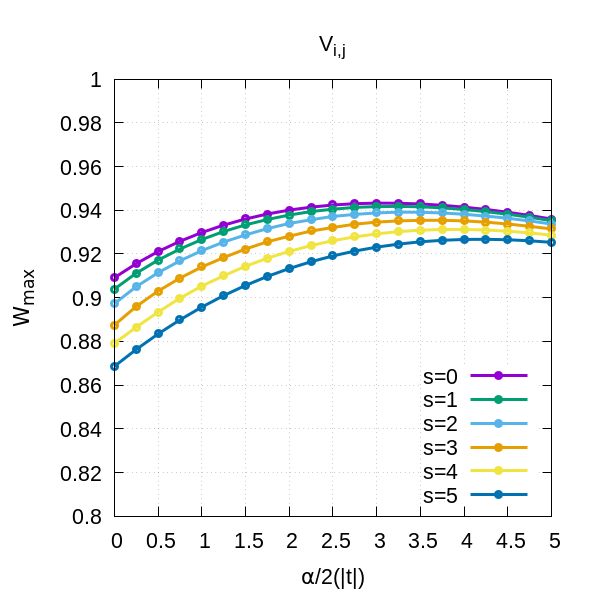
\includegraphics[scale=0.3]{Wmax_vs_xrep0vn.png}
		\end{minipage}
		\caption{\label{fig_v1n} Maximal weight (W$_{max}$) for each state as a function of repulsion calculated with two models: only considering repulsion between consecutive holes (left) and considering repulsion between all the holes as function of distance (right). }
	\end{figure}
	
	\subsection{Impact on $J_m$}
	\begin{figure}[h!]
		\centering
		\hspace{-2cm}
		\begin{minipage}{0.4\textwidth}
			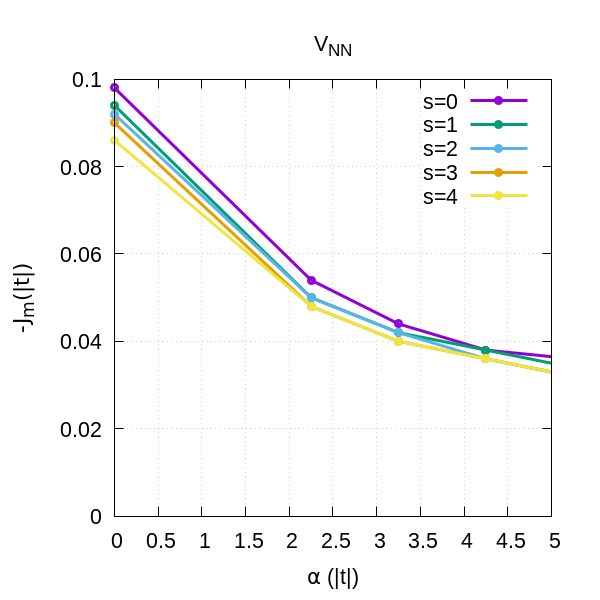
\includegraphics[scale=0.3]{J_vs_xrepv1.png}
		\end{minipage}
		\hspace{2cm}
		\begin{minipage}{0.4\textwidth}
			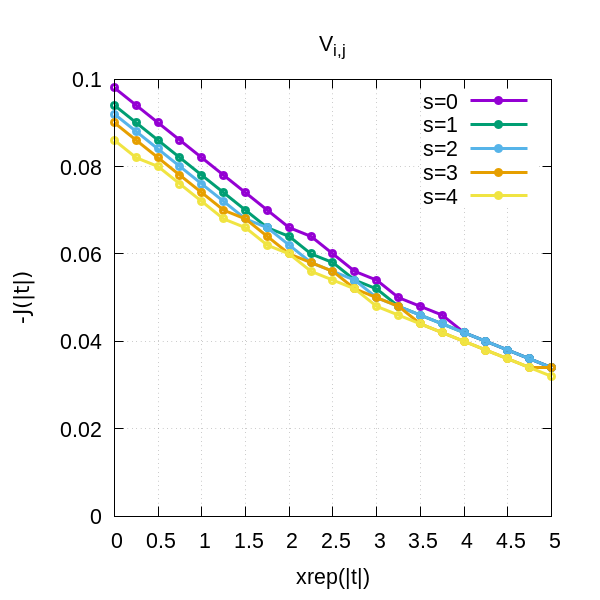
\includegraphics[scale=0.3]{J_vs_xrepvn.png}
		\end{minipage}
		\caption{\label{fig_jv1n} Value of $J$ for which the maximal weight is reached ($J_m$) as a function of repulsion calculated with two models: only considering repulsion between consecutive holes (left) and considering repulsion between all the holes as function of distance (right). }
	\end{figure}

	In order to rationalize this decrease in $J_m$ with $\alpha$, we propose the
	following explanation.  Repulsion decreases the kinetic energy of the system
	as it constrains the movement of holes, this will have a direct impact in
	the magnitude of the effect of $t$. As we pointed before there is a
	competition between $J$ (which favors antiferromagnetic coupling) and $t$
	(which favors ferromagnetic coupling), so this negative impact of repulsion
	on the effect of $t$ will cause that for even smaller values of $J$ the
	antiferromagnetic coupling becomes stronger and makes the weight falls
	abruptly as discussed in section 3.1.1.  Therefore the maximal value of
	weight is reached for smaller values of $J$ and $J_m$ is smaller as shown in
	figure \ref{fig_jv1n} in which it is possible to see the value of $J$ for
	which the maximal weight is reached for several values of $\alpha$ and also
	for the two models explained above. Note that no significants differences
	are found between the two types of repulsion.

	%\subsection{RSRG}

	\subsection{Conclusions}

	For reasonable values of repulsion the projections are good and the weight
	has a maximal value for $\alpha$ around 2.25$|t|$ with $J=0.064|t|$.
	
	\section{Results of $J_{eff}$}

	\subsection{Influence of the number of sites}
	\begin{figure}[h!]
		\centering
		\hspace{-2cm}
		\begin{minipage}{0.4\textwidth}
			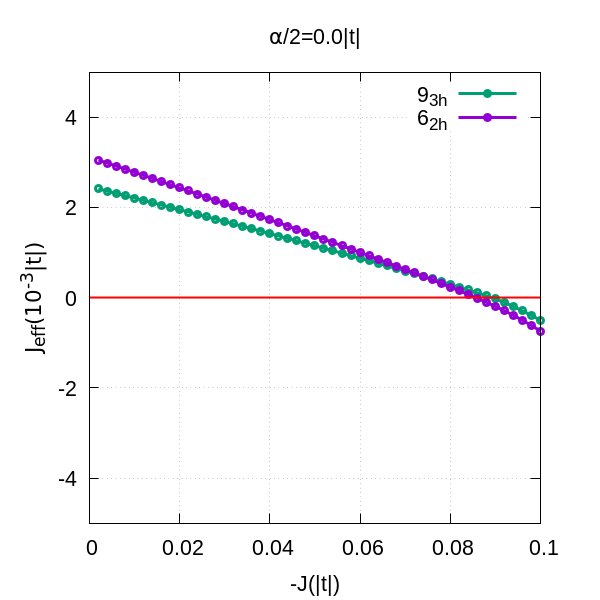
\includegraphics[scale=0.3]{Jeff_vs_J_sites_3-xrep-0.png}
		\end{minipage}
		\hspace{2cm}
		\begin{minipage}{0.4\textwidth}
			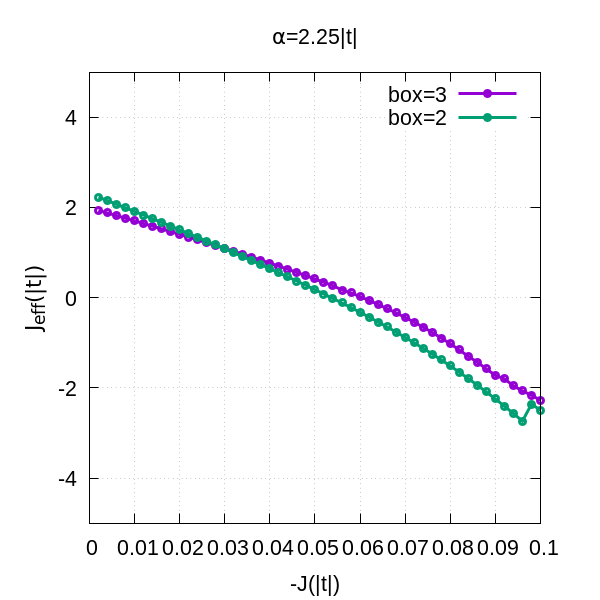
\includegraphics[scale=0.3]{Jeff_vs_J_sites_3-xrep-225.png}
		\end{minipage}
		\caption{\label{fig_arj} Value of $J_{eff}$ as a function of $J$ for $\alpha=0|t|$ (left) and $\alpha=2.25|t|$ (right). }
	\end{figure}

	Figure \ref{fig_arj} shows the values of $J_{eff}$ obtained by fitting the
	effective hamiltonian to te model hamiltonian, for 6$_{2h}$ and 9$_{3h}$, and
	for two different values of $\alpha$ in an interval in which the
	wavefunction has a good projection. There is an interval in which $J_{eff}$
	becomes antiferromagnetic (below the red line). As it is observed the values
	for both systems are pretty close, so in this range of values $J_{eff}$
	seems to be transferable.

	

	
	\subsection{Influence of hole repulsion}
		\begin{figure}[h!]
		\centering
		\hspace{-2cm}
		\begin{minipage}{0.4\textwidth}
			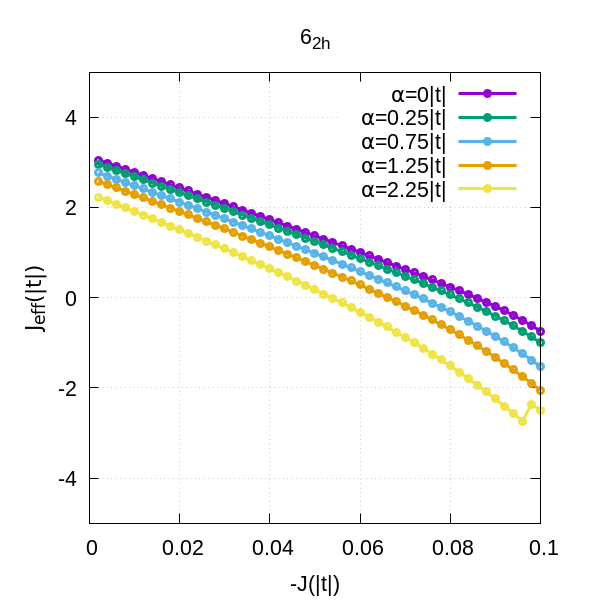
\includegraphics[scale=0.3]{Jeff_vs_J_ar2.png}
		\end{minipage}
		\hspace{2cm}
		\begin{minipage}{0.4\textwidth}
			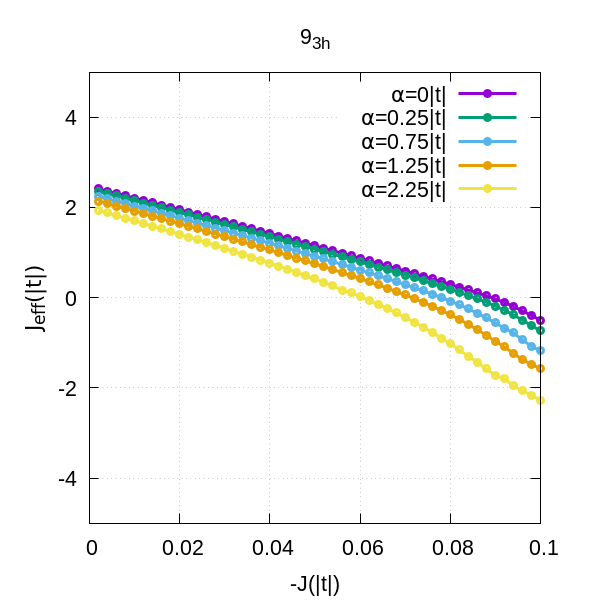
\includegraphics[scale=0.3]{Jeff_vs_J_ar3.png}
		\end{minipage}
		\caption{\label{fig_arj1} Value of $J_{eff}$ as a function of $J$ for 6$_{2h}$ (left) and 6$_{2h}$ (right). }
	\end{figure}
	
	\begin{figure}[h!]
		\centering
		\hspace{-2cm}
		\begin{minipage}{0.4\textwidth}
			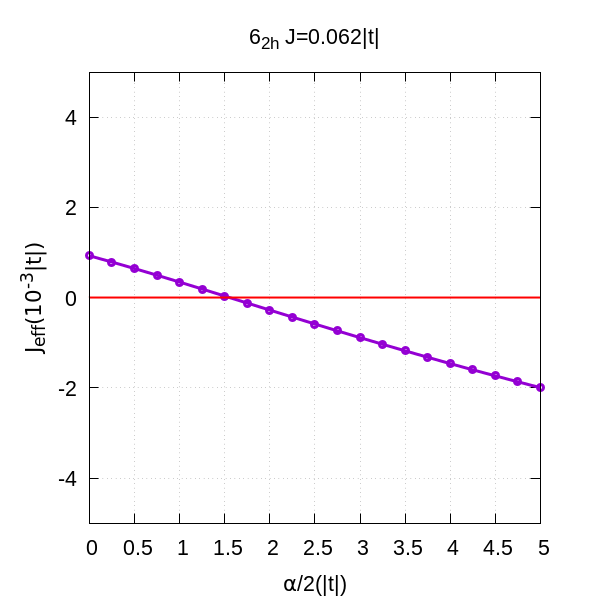
\includegraphics[scale=0.3]{Jeff_vs_xrep_ar2.png}
		\end{minipage}
		\hspace{2cm}
		\begin{minipage}{0.4\textwidth}
			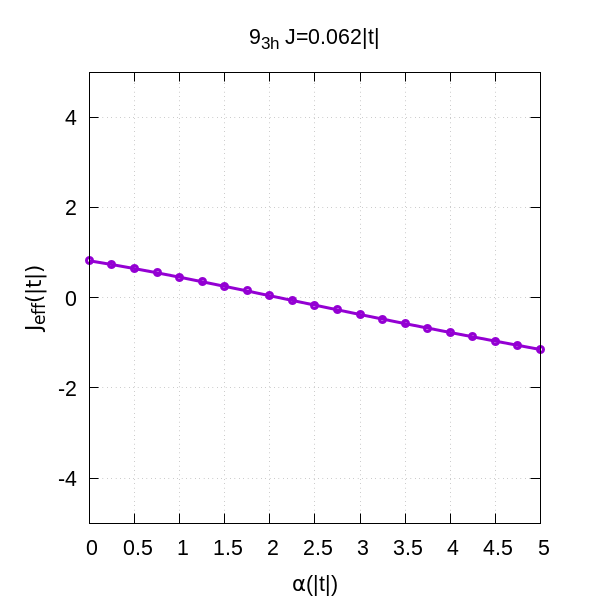
\includegraphics[scale=0.3]{Jeff_vs_xrep_ar3.png}
		\end{minipage}
		\caption{\label{fig_arxrep} Value of $J_{eff}$ as a function of $\alpha$ for 6$_{2h}$ (left) and 6$_{2h}$ (right). in both cases $J=0.062 |t|$ }
	\end{figure}

	In order to understand the influence of repulsion on $J_{eff}$, we have
	performed the fit to obtain $J_{eff}$ for several values of $\alpha$ as
	represented in figure \ref{fig_arj1}. Intersetingly, the $J_{eff}$ seems to
	vary linearly with $J$ with a different slope for the ferromagnetic part and
	the anti-ferromagnetic part. This suggests a possible existance of a phase
	transition.

	Upon increasing the repulsion, $J_{eff}$ goes faster to antiferromagnetic
	values. This results is ilustrated in figure \ref{fig_arxrep} in which
	$J_{eff}$ is represented as a function of repulsion for $J=0.062|t|$. This
	is a very interesting result which we have not yet been able to explain.
   \section{Spectrum}
   
   \begin{table}[H]
   \label{spectrum}
	\caption{Comparison of low energy spectrum calculated by double change hamiltonian and our model hamiltonian }
	\begin{center}
		\begin{tabular}{|c|c|c|c|}
			\hline
			 spin & $E_{DEHam}(10^{-3}|t|)$ & $E_{MHam}(10^{-3}|t|)$ & $\Delta E(10^{-3}|t|)$ \\
			\hline
			5 & 0  & 0  & 0  \\
			\hline
			4 & -2.69825 & -3.184 & 0.48575 \\
			\hline
			3 & -4.85685 & -5.220 & 0.36315 \\
			\hline
			2 & -6.47580 & -6.565 & 0.08920 \\
			\hline
			1 & -7.55510 & -7.395 & 0.1601 \\
			\hline
			0 & -8.09475 & -7.793 & 0.3017  \\
			\hline
			%$J_2-J_1$ & 0.072 & 0.024 & 0.104 \\
			%\hline
		\end{tabular}
	\end{center}
\end{table}
In the tabe \ref{spectrum} is showed the low energy spectrum calculated with double exchange hamiltonian and with our hamiltonian, this allows us to have a measurement of how good the model reproduce the system. As it is possible to see there are a reasonable agreement for both models. The state $S=5$ is taken as a reference so it is always zero and the the others values shows the energy gap between them and $S=5$
	\end{chapter} %{Discussion}
	
	\chapter*{ General Conclusions}
	Analyzing this kind of systems is a big challenge because of the size, computational cost, and the amount of information to process even more when it comes to larger amount of sites. In this work we have diagonalized the double exchange hamiltonian for $6_{2h}$ and $9_{3h}$ (calculations for $12_{4h}$ are still running), for several values of repulsions (within two models) and 100 values of $J$, this sorts an amount of information impossible to show in a limited extension repport but useful for understanding the physics of the problem. 
	
	As its have been presented the boxes model trhows some good results, which is a good new, as it reduce the size in a considerable way. It is possible to find some ranges of the parameters in which the double exchange wavefunction has an excellent projection in the model space, mainly (with some variations) when $0.6 < J < 0.1|t|$, $1.5|t| \leq \alpha \slash 2 \leq 2.5$. The incorporation of repulsion its been proven to be a good factor as it improves the projections.
	
	By the other hand, the values of $J_{eff}$ calculated in the interval of $J$ in which there is a good projection and the low energy spectrum, show that Heisemberg hamiltonian can reproduce well the coupling between the boxes. This values semm to have a linear dependence of $J$ with a change of phase when it turns unto antiferromagnetic region, this and its apparently transferability (to corraborate with bigger systems) could allow to have, with a reasonable accuracy, an analitical expression of $J_{eff}$ as a function of $J$ by fitting. Actually this antiferromagnetic coupling between the boxes is criticall for colossal magnetoresistance as the ground state is $S=0$ and the small values of $J_{eff}$ compared to $J$ makes the energy gap with the highest spin state to be very small and changable by applying a magnetic field. When the highest spin state becomes the ground state this favors electricall conductivity and this can explain its change even in orders of magnitude in the presence of a magnetic field. There is still a lot to understand and a lot of work to do but the perspective of this field are very exciting.
	\addcontentsline{toc}{chapter}{Conclusions}
	%\end{chapter}
	\newpage
	\pagenumbering{roman}
	\renewcommand{\bibname}{References}
	%\chapter*{References}
		\bibliography{biblio} % Use the example bibliography file sample.bib
	\bibliographystyle{unsrt} % Plain referencing style
	\addcontentsline{toc}{chapter}{References}
		\pagenumbering{roman}
		\setcounter{page}{2}

\end{document}



%*************************************************************************
% Bibliographies
%*************************************************************************
%\printbibliography
\bibliography{biblio.bib} % Use the example bibliography file sample.bib
\bibliographystyle{plain} % Plain referencing style
